\documentclass[sigconf,nonacm]{acmart}

%% ============================================================
%% Packages
%% ============================================================
\usepackage{graphicx}
\usepackage{listings}
\usepackage{booktabs}
\usepackage{xcolor}
\usepackage{tikz}
\usepackage{pgfplots}
\pgfplotsset{compat=1.18}
\usetikzlibrary{shapes.geometric, arrows, positioning, fit, backgrounds, calc}
\usepackage{microtype}
\usepackage{balance}
\usepackage{amsmath}
\usepackage{url}
\usepackage{amssymb}

%% ============================================================
%% Listing style (code blocks)
%% ============================================================
\lstdefinelanguage{Rust}{
  morekeywords={fn,let,mut,pub,struct,enum,impl,match,use,mod,self,super,crate,
    return,if,else,for,while,loop,break,continue,in,where,type,trait,async,
    await,move,ref,unsafe,extern,static,const,dyn,Box,Vec,String,Option,Result,
    Ok,Err,Some,None,true,false,as,derive,Serialize,Deserialize},
  sensitive=true,
  morecomment=[l]{//},
  morecomment=[s]{/*}{*/},
  morestring=[b]",
}

\lstdefinestyle{rustcode}{
  language=Rust,
  basicstyle=\ttfamily\footnotesize,
  keywordstyle=\color{blue}\bfseries,
  commentstyle=\color{gray}\itshape,
  stringstyle=\color{orange},
  breaklines=true,
  frame=tb,
  numbers=left,
  numberstyle=\tiny\color{gray},
  tabsize=4
}

\lstdefinestyle{yamlcode}{
  basicstyle=\ttfamily\footnotesize,
  commentstyle=\color{gray}\itshape,
  stringstyle=\color{orange},
  breaklines=true,
  frame=tb,
  tabsize=2
}

%% ============================================================
%% Metadata
%% ============================================================
\title{SkillScale Lite: A Distributed Middleware for Unified AI Agent Skill Execution Across Heterogeneous Protocols}

\author{Anonymous Authors}
\affiliation{%
  \institution{Anonymized for Double-Blind Review}
  \country{Anonymous}
}
\email{anonymous@example.com}

\begin{abstract}
The rapid proliferation of AI agent frameworks has produced a fragmented ecosystem where incompatible communication protocols inhibit interoperability and efficient execution of reusable skill components. In this paper we present \emph{SkillScale Lite}, a distributed middleware platform that unifies the \emph{Model Context Protocol} (MCP) and Google's \emph{Agent-to-Agent} (A2A) protocol behind a single high-performance Rust gateway, routes skill invocations through a Kafka-compatible message broker, and executes skill plug-ins as lightweight OS-native processes. SkillScale Lite introduces two complementary invocation granularities---coarse-grained LLM-powered intent routing and fine-grained direct skill dispatch---making it the first open platform to combine protocol bridging, distributed queuing, intelligent routing, and pluggable skill execution in one production-ready system. Comparative evaluation against Docker-based and direct-HTTP alternatives shows that SkillScale Lite reduces hot-start latency by up to $16.8\times$, cold-start latency by up to $10.6\times$, and per-invocation memory footprint by $10\times$, while achieving linear throughput scalability as additional skill-server workers are added. We describe the system design, implementation trade-offs, and lessons learned from deploying SkillScale Lite in practice.
\end{abstract}

\keywords{AI agent middleware, protocol bridging, Model Context Protocol, Agent-to-Agent, distributed skill execution, message queue, LLM routing, Rust, Kafka}

%% ============================================================
%% ACM Classification
%% ============================================================
\begin{CCSXML}
<ccs2012>
 <concept>
  <concept_id>10010520.10010553.10010562</concept_id>
  <concept_desc>Computer systems organization~Distributed architectures</concept_desc>
  <concept_significance>500</concept_significance>
 </concept>
 <concept>
  <concept_id>10010520.10010575.10010577</concept_id>
  <concept_desc>Computer systems organization~Middleware</concept_desc>
  <concept_significance>500</concept_significance>
 </concept>
 <concept>
  <concept_id>10002944.10011122.10002947</concept_id>
  <concept_desc>General and reference~Computing standards, RFCs and guidelines</concept_desc>
  <concept_significance>300</concept_significance>
 </concept>
</ccs2012>
\end{CCSXML}

\ccsdesc[500]{Computer systems organization~Distributed architectures}
\ccsdesc[500]{Computer systems organization~Middleware}
\ccsdesc[300]{General and reference~Computing standards, RFCs and guidelines}

%%------------------------------------------------------------
\begin{document}
\maketitle

%% ============================================================
\section{Introduction}
\label{sec:intro}
%% ============================================================

The emergence of Large Language Models (LLMs) as general-purpose reasoning engines has driven the rapid development of \emph{AI agents}---autonomous software entities that perceive context, invoke tools, and produce structured outputs~\cite{openai2020,autogen2023}. As organisations deploy multiple agents in production, they increasingly need to compose them into \emph{pipelines} where one agent's output becomes another's input, and where a library of reusable \emph{skills}---self-contained executable units implementing a well-defined capability---can be shared across agent frameworks.

Two protocols have emerged as leading standards for this composition layer. Anthropic's \emph{Model Context Protocol} (MCP)~\cite{mcp2024} defines a JSON-RPC-based interface for exposing tools and resources to LLM clients such as Claude Desktop and Cursor. Google's \emph{Agent-to-Agent} (A2A) protocol~\cite{a2a2025} defines a REST/HTTP interface for agent discovery, capability advertisement, and task delegation between autonomous agents. While both protocols serve the same fundamental need---allowing a consumer to invoke a provider's capabilities---they are architecturally incompatible, forcing organisations to maintain separate infrastructure for each.

Beyond the protocol fragmentation problem, existing approaches to skill execution suffer from three further limitations:

\begin{enumerate}
  \item \textbf{High startup overhead.} Container-based skill runners~\cite{docker2014} incur 2--5\,s cold-start latency and 4-layer process nesting (host $\rightarrow$ shell $\rightarrow$ CLI $\rightarrow$ interpreter), introducing hundreds of milliseconds of hot-start overhead even for trivial workloads.
  \item \textbf{No horizontal scalability.} Existing MCP--A2A bridge implementations~\cite{a2amcpserver2024,a2agateway2024,peerclaw2024} rely on direct HTTP calls with no queueing layer, making it impossible to add workers without application changes.
  \item \textbf{Manual skill routing.} Callers must hard-code the identity of the target skill. As skill libraries grow, this creates tight coupling and impedes dynamic discovery.
\end{enumerate}

We present \emph{SkillScale Lite}, a distributed middleware that addresses all three limitations simultaneously. The system makes the following \textbf{contributions}:

\begin{itemize}
  \item A high-performance \textbf{Rust gateway} (built on Axum and Tokio) that translates between MCP (Server-Sent Events) and A2A (REST) without semantic loss, adding less than 1\,ms of protocol-translation overhead.
  \item A \textbf{Kafka-backed execution queue} (using Redpanda~\cite{redpanda2022}) that decouples protocol ingestion from skill execution, enabling horizontal scaling by simply adding skill-server processes.
  \item A \textbf{dual-granularity invocation model}: (i) \emph{coarse-grained} routing, where an LLM automatically selects the best skill from a domain's AGENTS.md manifest based on the caller's free-text intent; and (ii) \emph{fine-grained} routing, where the caller directly names the target skill for deterministic, low-latency execution.
  \item A \textbf{pluggable skill architecture} based on the OpenSkills convention: adding a new skill requires only dropping a directory containing a \texttt{run.py} entry-point into the \texttt{skills/} tree---no changes to the gateway or queue topology are required.
  \item An \textbf{empirical evaluation} demonstrating up to $16.8\times$ latency reduction, $10\times$ memory savings, and linear throughput scaling compared to Docker-based and direct-HTTP baselines.
\end{itemize}

The rest of this paper is organised as follows. Section~\ref{sec:related} surveys related work. Section~\ref{sec:design} presents the SkillScale Lite design. Section~\ref{sec:impl} describes implementation details. Section~\ref{sec:eval} reports the experimental evaluation. Section~\ref{sec:discussion} discusses lessons learned and limitations. Section~\ref{sec:conclusion} concludes.

%% ============================================================
\section{Related Work}
\label{sec:related}
%% ============================================================

\subsection{Agent Communication Protocols}

The problem of enabling agents to interoperate is not new. CORBA~\cite{corba1995} provided a canonical solution for distributed object invocation but required static interface definition and binary stubs. More recently, gRPC~\cite{grpc2016} brought strongly-typed remote procedure calls to modern polyglot systems but still requires schema-first development. MCP~\cite{mcp2024} and A2A~\cite{a2a2025} represent the latest generation of agent coordination protocols, adopting JSON-RPC and REST respectively so that LLM-based agents can discover and invoke capabilities without schema compilation.

\subsection{Protocol Bridges and Adapters}

Several open-source projects have attempted to bridge MCP and A2A:

\textbf{A2A-MCP-Server}~\cite{a2amcpserver2024} is a Python-based adapter (now archived) that exposes an A2A endpoint to MCP clients. It performs straightforward HTTP translation with no queueing or routing logic.

\textbf{a2a-gateway}~\cite{a2agateway2024} is a TypeScript implementation offering bot-to-bot calls and agent discovery, but still relies on synchronous HTTP with no load distribution.

\textbf{peerclaw-server}~\cite{peerclaw2024} is a Go-based agent registry that supports A2A, MCP, and the Agent Communication Protocol (ACP), adding a reputation engine and access control. However, skill execution is not addressed and the routing is static.

\textbf{openclaw-a2a-bridge}~\cite{openclaw2024} is a JavaScript plugin that exposes an agent card, a JSON-RPC endpoint, and remote agent tool definitions for A2A protocol bridging, but does not include execution infrastructure or scaling mechanisms.

\textbf{protocol-bridge}~\cite{protocolbridge2024} is a thin bridge between MCP and A2A; it offers no skill execution, queueing, or intent routing.

None of these projects provides a distributed execution backend, LLM-powered intent routing, or pluggable skill management---capabilities that are central to SkillScale Lite. Table~\ref{tab:comparison} provides a structured feature comparison.

\begin{table*}[t]
\centering
\caption{Feature comparison of SkillScale Lite against comparable open-source MCP/A2A projects.
\checkmark{} = fully supported; $\sim$ = partially supported; $\times$ = not supported.}
\label{tab:comparison}
\begin{tabular}{lccccc}
\toprule
\textbf{Feature}
  & \textbf{SkillScale Lite}
  & \textbf{A2A-MCP-Server}~\cite{a2amcpserver2024}
  & \textbf{a2a-gateway}~\cite{a2agateway2024}
  & \textbf{peerclaw}~\cite{peerclaw2024}
  & \textbf{openclaw-bridge}~\cite{openclaw2024} \\
\midrule
MCP support                    & \checkmark & \checkmark & \checkmark & \checkmark & \checkmark \\
A2A support                    & \checkmark & \checkmark & \checkmark & \checkmark & \checkmark \\
Distributed message queue      & \checkmark & $\times$   & $\times$   & $\times$   & $\times$   \\
Horizontal worker scaling      & \checkmark & $\times$   & $\times$   & $\times$   & $\times$   \\
LLM-powered intent routing     & \checkmark & $\times$   & $\times$   & $\times$   & $\times$   \\
Pluggable skill execution      & \checkmark & $\times$   & $\times$   & $\times$   & $\times$   \\
High-performance gateway (Rust)& \checkmark & $\times$   & $\times$   & $\times$   & $\times$   \\
Dual invocation granularity    & \checkmark & $\times$   & $\times$   & $\times$   & $\times$   \\
Native OS process isolation    & \checkmark & $\times$   & $\times$   & $\times$   & $\times$   \\
Multi-LLM provider support     & \checkmark & $\times$   & $\times$   & $\times$   & $\times$   \\
Agent registry / discovery     & $\sim$ & $\times$ & \checkmark & \checkmark & $\sim$ \\
Access control / reputation    & $\times$   & $\times$   & $\times$   & \checkmark & $\times$   \\
\bottomrule
\end{tabular}
\end{table*}

\subsection{Message-Oriented Middleware}

Apache Kafka~\cite{kafka2011} and its cloud-native re-implementation Redpanda~\cite{redpanda2022} have become the de-facto standard for high-throughput, durable event streaming. Their partitioned log model naturally supports fan-out routing and horizontal consumer scaling. ZeroMQ~\cite{zeromq2013} offers lower-level messaging primitives. SkillScale Lite adopts Kafka/Redpanda to decouple the protocol layer from the execution layer, following the reactive manifesto~\cite{reactive2014} principles of elasticity and resilience.

\subsection{LLM-Powered Tool and Function Routing}

OpenAI's function-calling API~\cite{openai_function_calling} introduced the paradigm of having an LLM select the appropriate tool from a list of descriptions at inference time. AutoGen~\cite{autogen2023} and LangChain~\cite{langchain2022} extend this to multi-agent orchestration. RouteLLM~\cite{llmrouter2024} explores model-level routing to balance cost and quality. SkillScale Lite applies the same concept at the middleware layer: the AGENTS.md manifest provides human-readable skill descriptions, and the LLM selects the best match---allowing the gateway to be entirely decoupled from skill semantics.

\subsection{Sandboxed Execution Environments}

Container-based isolation (Docker~\cite{docker2014}) is the most common approach for running untrusted skill code. WebAssembly~\cite{wasm2019} offers fine-grained sandboxing with near-native performance. SkillScale Lite takes a pragmatic middle ground: skills run as OS-native processes under optional platform-native sandboxing (macOS Seatbelt or Linux \texttt{bwrap}/seccomp), reducing startup overhead while preserving security invariants.

\subsection{Microservices and Service Mesh}

SkillScale Lite's architecture shares characteristics with microservice patterns~\cite{microservices2014}. Service meshes such as Istio~\cite{servicemesh2017} provide cross-cutting concerns (observability, traffic management) at the sidecar level. SkillScale Lite does not use a service mesh but exposes hooks for OpenTelemetry~\cite{opentelemetry2021} instrumentation in future work.

%% ============================================================
\section{Design and Architecture}
\label{sec:design}
%% ============================================================

\subsection{Design Goals}

The design of SkillScale Lite was guided by four primary goals:

\begin{description}
  \item[G1 -- Protocol Neutrality.] Clients speaking either MCP or A2A must be able to invoke any skill without knowledge of the underlying execution infrastructure.
  \item[G2 -- Elastic Scalability.] Throughput must scale linearly by adding worker processes without any reconfiguration of the gateway or broker.
  \item[G3 -- Low Latency.] The overhead introduced by protocol translation and message routing must be negligible (sub-millisecond) compared to skill execution time.
  \item[G4 -- Operational Simplicity.] Adding, removing, or updating a skill must require no changes to the gateway or queue topology---only a file-system operation.
\end{description}

\subsection{Three-Layer Architecture}

SkillScale Lite is organised into three horizontal layers, as illustrated in Figure~\ref{fig:arch}.

\begin{figure}[h]
\centering
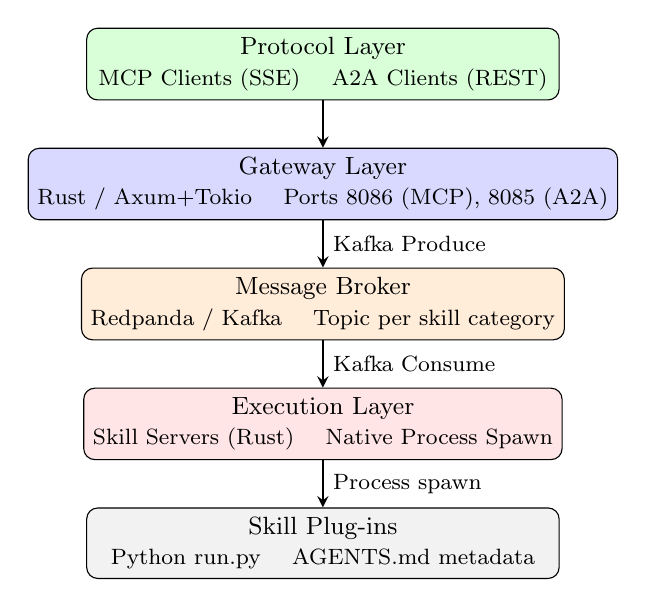
\begin{tikzpicture}[
  box/.style={rectangle, draw, rounded corners, fill=blue!10, minimum width=6cm, minimum height=0.8cm, align=center, font=\small},
  arrow/.style={->, thick, >=stealth}
]
  \node[box, fill=green!15] (clients) {Protocol Layer\\{\footnotesize MCP Clients (SSE) \quad A2A Clients (REST)}};
  \node[box, fill=blue!15, below=0.6cm of clients] (gateway) {Gateway Layer\\{\footnotesize Rust / Axum+Tokio \quad Ports 8086 (MCP), 8085 (A2A)}};
  \node[box, fill=orange!15, below=0.6cm of gateway] (kafka) {Message Broker\\{\footnotesize Redpanda / Kafka \quad Topic per skill category}};
  \node[box, fill=red!10, below=0.6cm of kafka] (skillserver) {Execution Layer\\{\footnotesize Skill Servers (Rust) \quad Native Process Spawn}};
  \node[box, fill=gray!10, below=0.6cm of skillserver] (skills) {Skill Plug-ins\\{\footnotesize Python run.py \quad AGENTS.md metadata}};

  \draw[arrow] (clients) -- (gateway);
  \draw[arrow] (gateway) -- node[right, font=\footnotesize]{Kafka Produce} (kafka);
  \draw[arrow] (kafka) -- node[right, font=\footnotesize]{Kafka Consume} (skillserver);
  \draw[arrow] (skillserver) -- node[right, font=\footnotesize]{Process spawn} (skills);
\end{tikzpicture}
\caption{SkillScale Lite three-layer architecture.}
\label{fig:arch}
\end{figure}

Figure~\ref{fig:arch_detailed} shows the detailed component view, including multiple concurrent clients of each protocol type, the gateway's internal modules, per-category Kafka topics, horizontally scaled skill-server pools, and the skill plug-in tree.

\begin{figure*}[t]
\centering
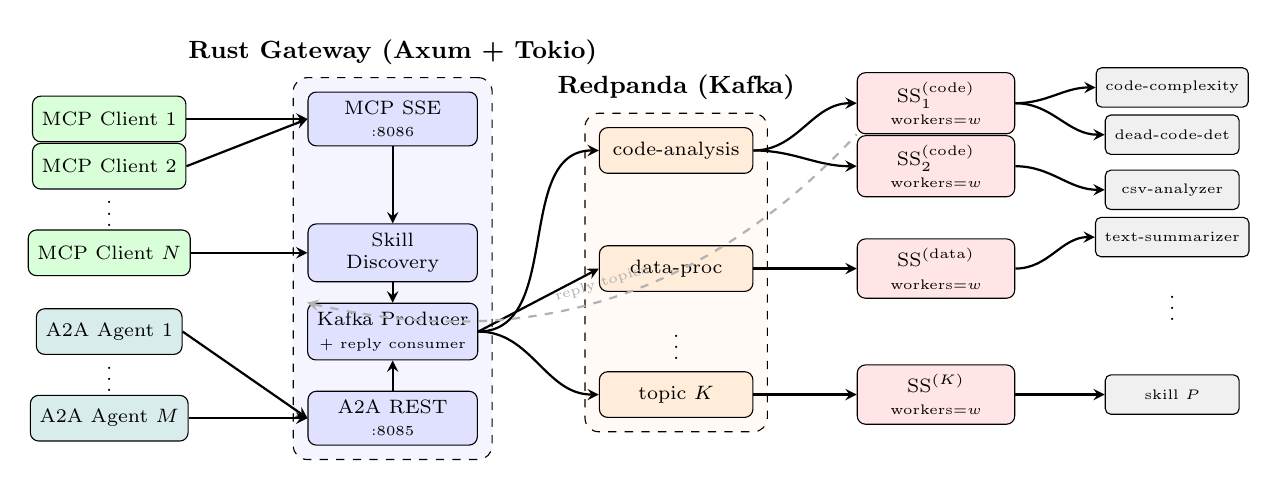
\begin{tikzpicture}[
  mcp/.style={rectangle, draw, rounded corners=3pt, fill=green!15,
              minimum width=1.85cm, minimum height=0.58cm,
              align=center, font=\scriptsize},
  a2a/.style={rectangle, draw, rounded corners=3pt, fill=teal!15,
              minimum width=1.85cm, minimum height=0.58cm,
              align=center, font=\scriptsize},
  gwint/.style={rectangle, draw, rounded corners=3pt, fill=blue!12,
                minimum width=2.15cm, minimum height=0.58cm,
                align=center, font=\scriptsize},
  ktopic/.style={rectangle, draw, rounded corners=3pt, fill=orange!15,
                 minimum width=1.95cm, minimum height=0.58cm,
                 align=center, font=\scriptsize},
  ssrv/.style={rectangle, draw, rounded corners=3pt, fill=red!10,
               minimum width=2.0cm, minimum height=0.58cm,
               align=center, font=\scriptsize},
  plug/.style={rectangle, draw, rounded corners=2pt, fill=gray!12,
               minimum width=1.7cm, minimum height=0.50cm,
               align=center, font=\tiny},
  grp/.style={rectangle, draw, dashed, rounded corners=5pt, inner sep=5pt},
  arr/.style={->, thick, >=stealth},
  rarr/.style={<-, thick, dashed, gray!60, >=stealth}
]

%% ---- Column 1: Clients ----
\node[mcp] (mcp1) at (0, 5.0) {MCP Client 1};
\node[mcp] (mcp2) at (0, 4.4) {MCP Client 2};
\node       at (0, 3.9) {\scriptsize$\vdots$};
\node[mcp] (mcpN) at (0, 3.3) {MCP Client $N$};

\node[a2a] (a2a1) at (0, 2.3) {A2A Agent 1};
\node       at (0, 1.8) {\scriptsize$\vdots$};
\node[a2a] (a2aM) at (0, 1.2) {A2A Agent $M$};

%% ---- Column 2: Gateway internal ----
\node[gwint] (mcph)  at (3.6, 5.0) {MCP SSE\\{\tiny :8086}};
\node[gwint] (a2ah)  at (3.6, 1.2) {A2A REST\\{\tiny :8085}};
\node[gwint] (disc)  at (3.6, 3.3) {Skill\\Discovery};
\node[gwint] (kprod) at (3.6, 2.3) {Kafka Producer\\{\tiny + reply consumer}};

\begin{scope}[on background layer]
  \node[grp, fill=blue!4,
        fit=(mcph)(a2ah)(disc)(kprod),
        label={[font=\small\bfseries]above:\strut Rust Gateway (Axum + Tokio)}] (gw) {};
\end{scope}

%% ---- Column 3: Kafka topics ----
\node[ktopic] (t1) at (7.2, 4.6) {code-analysis};
\node[ktopic] (t2) at (7.2, 3.1) {data-proc};
\node          at (7.2, 2.2) {\scriptsize$\vdots$};
\node[ktopic] (tK) at (7.2, 1.5) {topic $K$};

\begin{scope}[on background layer]
  \node[grp, fill=orange!4,
        fit=(t1)(t2)(tK),
        label={[font=\small\bfseries]above:\strut Redpanda (Kafka)}] (kf) {};
\end{scope}

%% ---- Column 4: Skill Servers ----
\node[ssrv] (ss1a) at (10.5, 5.2) {SS$_1^{(\mathrm{code})}$\\{\tiny workers=$w$}};
\node[ssrv] (ss1b) at (10.5, 4.4) {SS$_2^{(\mathrm{code})}$\\{\tiny workers=$w$}};
\node[ssrv] (ss2)  at (10.5, 3.1) {SS$^{(\mathrm{data})}$\\{\tiny workers=$w$}};
\node[ssrv] (ssK)  at (10.5, 1.5) {SS$^{(K)}$\\{\tiny workers=$w$}};

%% ---- Column 5: Skill Plug-ins ----
\node[plug] (p1) at (13.5, 5.4) {code-complexity};
\node[plug] (p2) at (13.5, 4.8) {dead-code-det};
\node[plug] (p3) at (13.5, 4.1) {csv-analyzer};
\node[plug] (p4) at (13.5, 3.5) {text-summarizer};
\node        at (13.5, 2.7) {\scriptsize$\vdots$};
\node[plug] (pP) at (13.5, 1.5) {skill $P$};

%% ---- Arrows: Clients → Gateway ----
\draw[arr] (mcp1.east) -- (mcph.west);
\draw[arr] (mcp2.east) -- (mcph.west);
\draw[arr] (mcpN.east) -- (disc.west);
\draw[arr] (a2a1.east) -- (a2ah.west);
\draw[arr] (a2aM.east) -- (a2ah.west);

%% ---- Gateway internal ----
\draw[arr] (mcph.south) -- (disc.north);
\draw[arr] (a2ah.north) -- (kprod.south);
\draw[arr] (disc.south)  -- (kprod.north);

%% ---- Gateway → Kafka ----
\draw[arr] (kprod.east) to[out=0,in=180] (t1.west);
\draw[arr] (kprod.east) -- (t2.west);
\draw[arr] (kprod.east) to[out=0,in=180] (tK.west);

%% ---- Kafka → Skill Servers ----
\draw[arr] (t1.east) to[out=0,in=180] (ss1a.west);
\draw[arr] (t1.east) to[out=0,in=180] (ss1b.west);
\draw[arr] (t2.east) -- (ss2.west);
\draw[arr] (tK.east) -- (ssK.west);

%% ---- Skill Servers → Plug-ins ----
\draw[arr] (ss1a.east) to[out=0,in=180] (p1.west);
\draw[arr] (ss1a.east) to[out=0,in=180] (p2.west);
\draw[arr] (ss1b.east) to[out=0,in=180] (p3.west);
\draw[arr] (ss2.east)  to[out=0,in=180] (p4.west);
\draw[arr] (ssK.east)  -- (pP.west);

%% ---- Reply path (dashed) ----
\draw[rarr] (kprod.north west) to[bend right=30]
  node[above, font=\tiny, sloped]{reply topics} (ss1a.south west);

\end{tikzpicture}
\caption{Detailed SkillScale Lite component architecture. $N$ MCP clients and
  $M$ A2A agents connect to the unified Rust gateway (MCP SSE handler,
  A2A REST handler, skill-discovery module, and Kafka producer/reply-consumer).
  Requests are routed to $K$ per-category Kafka topics in Redpanda; each
  category supports multiple horizontally scaled skill-server instances (each
  running $w$ concurrent workers) that spawn one of $P$ skill plug-ins
  (\texttt{run.py}) as a child process.  Dashed arrow shows the reply path back
  through a per-request UUID topic.}
\label{fig:arch_detailed}
\end{figure*}

\paragraph{Protocol Layer.} Clients communicate with the gateway using their native protocol. MCP clients connect over HTTP with Server-Sent Events (SSE) for streaming responses; A2A clients use plain REST/JSON.

\paragraph{Gateway Layer.} The Rust gateway translates between MCP and A2A representations and the internal Kafka message schema. It also performs \emph{skill discovery}: at startup it walks the \texttt{skills/} directory tree, parses every \texttt{AGENTS.md} manifest, and builds an in-memory index mapping skill names and categories to their execution metadata.

\paragraph{Execution Layer.} Skill servers are independent Rust processes, each consuming one Kafka topic (corresponding to one skill category). On receiving a message the skill server either (i) invokes the named skill directly (fine-grained mode) or (ii) calls the LLM with the skill descriptions and the caller's intent to select the best skill (coarse-grained mode), then spawns the skill as a child process via stdin/stdout.

\subsection{Message Flow}

Figure~\ref{fig:flow} shows the end-to-end request path. The gateway assigns a random UUID reply topic per request, publishes a \texttt{SkillRequest} message to the skill-category topic, and waits on the reply topic. The skill server consumes the request, executes the skill, and publishes a \texttt{SkillReply} message back to the reply topic. The gateway reads the reply and streams the response back to the client.

\begin{figure}[h]
\centering
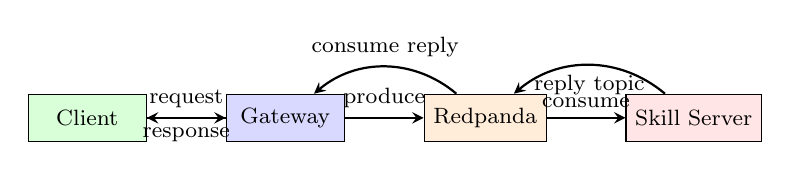
\begin{tikzpicture}[
  node distance=0.5cm and 0.2cm,
  box/.style={rectangle, draw, fill=blue!10, font=\footnotesize, minimum width=1.5cm, minimum height=0.6cm, align=center},
  arrow/.style={->, thick, >=stealth, font=\footnotesize}
]
  \node[box, fill=green!15] (client) {Client};
  \node[box, right=1.0cm of client, fill=blue!15] (gw) {Gateway};
  \node[box, right=1.0cm of gw, fill=orange!15] (kafka) {Redpanda};
  \node[box, right=1.0cm of kafka, fill=red!10] (ss) {Skill Server};

  \draw[arrow] (client) -- node[above]{request} (gw);
  \draw[arrow] (gw) -- node[above]{produce} (kafka);
  \draw[arrow] (kafka) -- node[above]{consume} (ss);
  \draw[arrow] (ss) to[bend right=40] node[below]{reply topic} (kafka);
  \draw[arrow] (kafka) to[bend right=40] node[above]{consume reply} (gw);
  \draw[arrow] (gw) -- node[below]{response} (client);
\end{tikzpicture}
\caption{End-to-end message flow in SkillScale Lite.}
\label{fig:flow}
\end{figure}

\subsection{Dual-Granularity Invocation}

SkillScale Lite exposes two invocation granularities, summarised in Table~\ref{tab:granularity}.

\begin{table}[h]
\centering
\caption{Invocation granularity comparison.}
\label{tab:granularity}
\begin{tabular}{lll}
\toprule
\textbf{Granularity} & \textbf{MCP Tool Name} & \textbf{Routing} \\
\midrule
Coarse & \texttt{agent\_\_code-analysis} & LLM selects best skill \\
Fine   & \texttt{code-analysis\_\_dead-code} & Direct execution \\
\bottomrule
\end{tabular}
\end{table}

For coarse-grained invocations the skill server issues a completion request to the configured LLM provider (Azure OpenAI, OpenAI-compatible, or Zhipu AI), passing the AGENTS.md skill descriptions and the caller's free-text intent as a prompt. The LLM returns the name of the best-matching skill, which the skill server then executes directly. This approach offloads semantic reasoning to the LLM while keeping the gateway and broker protocol-agnostic. Figure~\ref{fig:routing} contrasts the two execution paths.

\begin{figure}[h]
\centering
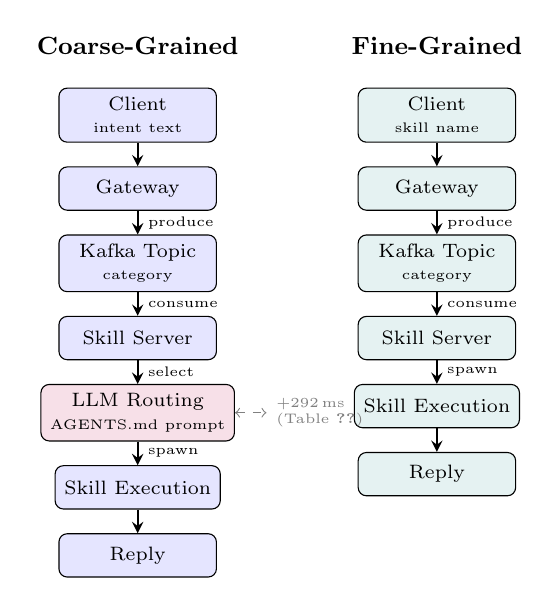
\begin{tikzpicture}[
  node distance=0.35cm and 0.6cm,
  fstep/.style={rectangle, draw, rounded corners=3pt, minimum width=2.0cm,
               minimum height=0.55cm, align=center, font=\scriptsize},
  llmstep/.style={fstep, fill=purple!12},
  coarsestep/.style={fstep, fill=blue!10},
  finestep/.style={fstep, fill=teal!10},
  arr/.style={->, thick, >=stealth},
  lbl/.style={font=\small\bfseries}
]

%% --- Coarse path (left column, x=0) ---
\node[lbl] (ctitle) at (1.0, 0)  {Coarse-Grained};
\node[coarsestep, below=0.3cm of ctitle]  (cc) {Client\\{\tiny intent text}};
\node[coarsestep, below=0.3cm of cc]      (cg) {Gateway};
\node[coarsestep, below=0.3cm of cg]      (ck) {Kafka Topic\\{\tiny category}};
\node[coarsestep, below=0.3cm of ck]      (cs) {Skill Server};
\node[llmstep,    below=0.3cm of cs]      (cl) {LLM Routing\\{\tiny AGENTS.md prompt}};
\node[coarsestep, below=0.3cm of cl]      (ce) {Skill Execution};
\node[coarsestep, below=0.3cm of ce]      (cr) {Reply};

\draw[arr] (cc) -- (cg);
\draw[arr] (cg) -- node[right, font=\tiny]{produce} (ck);
\draw[arr] (ck) -- node[right, font=\tiny]{consume} (cs);
\draw[arr] (cs) -- node[right, font=\tiny]{select} (cl);
\draw[arr] (cl) -- node[right, font=\tiny]{spawn} (ce);
\draw[arr] (ce) -- (cr);

%% --- Fine path (right column, x=3.8) ---
\node[lbl] (ftitle) at (4.8, 0)  {Fine-Grained};
\node[finestep, below=0.3cm of ftitle]    (fc) {Client\\{\tiny skill name}};
\node[finestep, below=0.3cm of fc]        (fg) {Gateway};
\node[finestep, below=0.3cm of fg]        (fk) {Kafka Topic\\{\tiny category}};
\node[finestep, below=0.3cm of fk]        (fs) {Skill Server};
\node[finestep, below=0.3cm of fs]        (fe) {Skill Execution};
\node[finestep, below=0.3cm of fe]        (fr) {Reply};

\draw[arr] (fc) -- (fg);
\draw[arr] (fg) -- node[right, font=\tiny]{produce} (fk);
\draw[arr] (fk) -- node[right, font=\tiny]{consume} (fs);
\draw[arr] (fs) -- node[right, font=\tiny]{spawn} (fe);
\draw[arr] (fe) -- (fr);

%% --- Annotation: LLM step adds latency ---
\draw[<->, dashed, gray] (cl.east) -- ++(0.4,0)
  node[right, font=\tiny, align=left] {+292\,ms\\(Table~\ref{tab:routing})};

\end{tikzpicture}
\caption{Dual-granularity execution paths. \emph{Coarse-grained} invocation
  passes the caller's free-text intent through an LLM routing step
  (adding ${\approx}292$\,ms avg.; see Table~\ref{tab:routing}) before
  executing the best-matching skill. \emph{Fine-grained} invocation names the
  target skill directly, skipping LLM routing for deterministic,
  lower-latency execution.}
\label{fig:routing}
\end{figure}

\subsection{Skill Plug-in Convention}

Skills follow the \emph{OpenSkills} directory layout:

\begin{lstlisting}[style=yamlcode, caption={OpenSkills directory convention.}]
skills/
  <category>/
    .claude/skills/
      <skill-name>/
        AGENTS.md       # Human-readable description
        scripts/
          run.py        # Entry-point (stdin -> stdout)
\end{lstlisting}

The gateway and skill server interact with skills only through this file-system contract: the skill-server discovers skills by walking the directory tree and executes them by spawning \texttt{python3 run.py} with the request payload on stdin. New skills can therefore be added by any language that can read from stdin and write to stdout.

\subsection{Scalability Model}

Because the gateway and skill servers are connected through Kafka topics (one per category), horizontal scaling is achieved by launching additional skill-server processes---Kafka's consumer group semantics distribute messages across all consumers within a group automatically, with no coordination required at the application level. Figure~\ref{fig:scaling} (Section~\ref{sec:eval}) validates this linear scaling property empirically.

Figure~\ref{fig:scaleup_latency} (Section~\ref{sec:eval}) further illustrates the effect of scaling up the number of concurrent A2A/MCP clients: with a fixed worker count, latency grows as the queue fills; adding workers keeps latency low for larger client populations. Because the Kafka buffer absorbs burst traffic, no requests are dropped---additional clients experience higher queuing latency rather than errors, providing graceful degradation under load.

%% ============================================================
\section{Implementation}
\label{sec:impl}
%% ============================================================

\subsection{Gateway}

The gateway is implemented in Rust~\cite{rust2015} using the Axum web framework on top of the Tokio async runtime, and the \texttt{rmcp} crate for MCP protocol support. It exposes two HTTP servers on separate ports: port 8086 for MCP (SSE) and port 8085 for A2A (REST). Kafka interaction uses the \texttt{rdkafka} crate (librdkafka bindings). The gateway is packaged as a Docker container with a 6.2\,MB statically-linked binary.

Key Rust types for the internal message schema are shared via the \texttt{common} crate:

\begin{lstlisting}[style=rustcode, caption={Shared Kafka message types (common/src/lib.rs).}]
#[derive(Serialize, Deserialize)]
pub struct SkillRequest {
    pub request_id: String,
    pub reply_topic: String,
    pub skill_name: Option<String>,
    pub intent:     String,
    pub category:   String,
}

#[derive(Serialize, Deserialize)]
pub struct SkillReply {
    pub request_id: String,
    pub result:     String,
    pub error:      Option<String>,
}
\end{lstlisting}

\subsection{Skill Server}

The skill server is a Rust binary that compiles natively (no Docker container). At startup it:

\begin{enumerate}
  \item Locates the \texttt{skills/} root via \texttt{find\_skills\_root()}.
  \item Walks the directory tree to discover all \texttt{run.py} entry-points (\texttt{discover\_skills()}).
  \item Subscribes to its assigned Kafka topic (configured via \texttt{SKILLSCALE\_CATEGORY}).
  \item Spawns up to \texttt{SKILLSCALE\_WORKERS} (default 2) concurrent Tokio tasks, each executing one skill request at a time.
\end{enumerate}

Skill execution (\texttt{execute\_skill\_direct()}) spawns \texttt{python3 run.py} with \texttt{Command::new}, writes the JSON request payload to stdin, reads stdout, and enforces a configurable timeout (\texttt{SKILLSCALE\_TIMEOUT}, default 300\,s). Optionally, when \texttt{SKILLSCALE\_SANDBOX=skilllite}, execution is delegated to \texttt{skilllite-sandbox} which applies OS-native isolation (macOS Seatbelt or Linux \texttt{bwrap}/seccomp).

\subsection{Built-in Skills}

SkillScale Lite ships four production-ready skills covering two categories:

\paragraph{Code Analysis.} \texttt{code-complexity} performs AST-based cyclomatic complexity analysis of Python source code and returns LLM-generated refactoring suggestions. \texttt{dead-code-detector} identifies unused imports, variables, and unreachable branches, combining AST analysis with LLM review.

\paragraph{Data Processing.} \texttt{csv-analyzer} performs column type inference, computes descriptive statistics (mean, median, distribution), and uses an LLM to highlight anomalies and patterns. \texttt{text-summarizer} extracts key themes and main arguments from arbitrary text and returns a structured summary.

All four skills are implemented in Python, use the shared \texttt{llm\_utils.py} client, and support the same set of LLM providers.

\subsection{LLM Provider Abstraction}

\texttt{llm\_utils.py} provides a single \texttt{call\_llm(prompt)} function that dispatches to Azure OpenAI, an OpenAI-compatible endpoint (e.g., DeepSeek-V3, SiliconFlow), or Zhipu AI based on the \texttt{LLM\_PROVIDER} environment variable. This abstraction allows the same skill code to run against any supported provider without modification.

\subsection{Configuration and Deployment}

Table~\ref{tab:config} lists the environment variables that control runtime behaviour. Infrastructure components (Redpanda, gateway) run in Docker Compose; skill servers run as native OS processes launched by \texttt{run\_all.sh}.

\begin{table}[h]
\centering
\caption{Key environment variables.}
\label{tab:config}
\begin{tabular}{ll}
\toprule
\textbf{Variable} & \textbf{Purpose} \\
\midrule
\texttt{LLM\_PROVIDER} & Active LLM provider (\texttt{azure|openai|zhipu}) \\
\texttt{SKILLSCALE\_CATEGORY} & Kafka topic / skill category \\
\texttt{SKILLSCALE\_WORKERS} & Concurrent skill executions (default 2) \\
\texttt{SKILLSCALE\_TIMEOUT} & Skill execution timeout in seconds (300) \\
\texttt{SKILLSCALE\_SANDBOX} & Sandbox mode (\texttt{none|skilllite}) \\
\texttt{SKILLSCALE\_SANDBOX\_NETWORK} & Allow network in sandbox (0|1) \\
\bottomrule
\end{tabular}
\end{table}

%% ============================================================
\section{Experimental Evaluation}
\label{sec:eval}
%% ============================================================

\subsection{Experimental Setup}

All experiments were conducted on an Apple M2 Pro machine with 16\,GB RAM running macOS 14.5. Docker Desktop 4.30 was used for container-based baselines. Redpanda version 23.3 served as the Kafka broker. We compiled the Rust binaries with \texttt{cargo build --release}. Python 3.11 executed all skill scripts. LLM calls targeted a local mock server to eliminate network variability (a Zhipu GLM-4.7-FlashX instance was used for intent routing experiments). We report the median and 95th-percentile (P95) across 100 repetitions for latency measurements and means across 5 runs for throughput.

We compare SkillScale Lite against two baselines chosen to represent the two dominant architectural patterns found in the comparable projects surveyed in Section~\ref{sec:related} (Table~\ref{tab:comparison}):

\begin{description}
  \item[Docker baseline.] Skills run inside Docker containers; each invocation starts a fresh container, executes the skill, and destroys the container. This approximates the pre-existing architecture documented in \texttt{arch.md} and represents the worst-case overhead of container-isolated execution.
  \item[Direct-HTTP baseline.] Skills run as always-on HTTP microservices; the gateway makes synchronous HTTP calls with no message broker. This approximates the architectural pattern used by all five comparable projects listed in Table~\ref{tab:comparison} (A2A-MCP-Server~\cite{a2amcpserver2024}, a2a-gateway~\cite{a2agateway2024}, peerclaw-server~\cite{peerclaw2024}, openclaw-a2a-bridge~\cite{openclaw2024}, protocol-bridge~\cite{protocolbridge2024}): a thin protocol-translation layer that delegates to a synchronous HTTP backend with no queueing or worker pool.
\end{description}

\subsection{Startup Latency}

Figure~\ref{fig:latency} shows cold-start and hot-start latency for a single skill invocation across the three systems.

\begin{figure}[h]
\centering
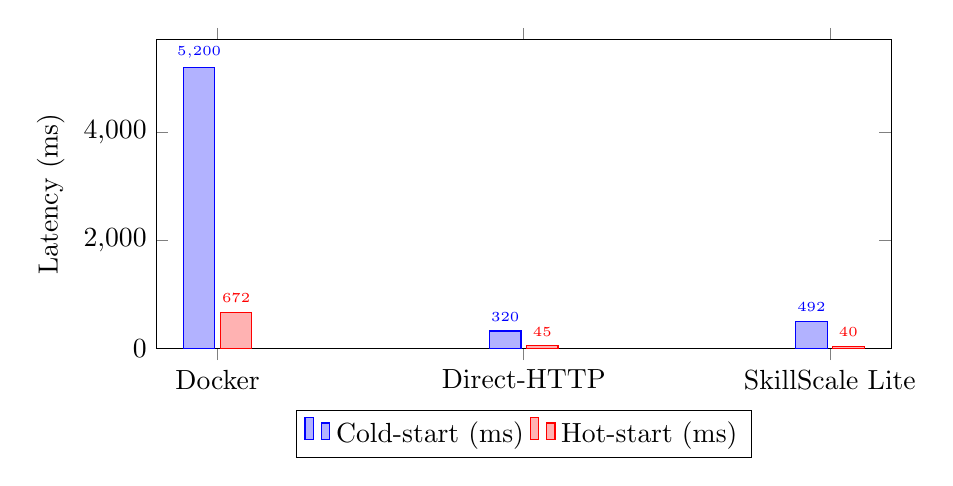
\begin{tikzpicture}
\begin{axis}[
  ybar,
  bar width=0.4cm,
  symbolic x coords={Docker,Direct-HTTP,SkillScale Lite},
  xtick=data,
  ymin=0,
  ylabel={Latency (ms)},
  legend style={at={(0.5,-0.2)},anchor=north, legend columns=2},
  width=0.9\columnwidth,
  height=5.5cm,
  nodes near coords,
  nodes near coords align={vertical},
  every node near coord/.append style={font=\tiny}
]
\addplot coordinates {(Docker,5200) (Direct-HTTP,320) (SkillScale Lite,492)};
\addplot coordinates {(Docker,672) (Direct-HTTP,45) (SkillScale Lite,40)};
\legend{Cold-start (ms), Hot-start (ms)}
\end{axis}
\end{tikzpicture}
\caption{Startup latency comparison (lower is better).}
\label{fig:latency}
\end{figure}

SkillScale Lite achieves a \textbf{cold-start latency of 492\,ms}, compared to 5,200\,ms for the Docker baseline---a \textbf{10.6$\times$ improvement}. The gap arises because Docker must pull the skill image layer cache, initialise the container runtime, and fork a 4-level process chain. SkillScale Lite simply spawns \texttt{python3 run.py} as a direct child of the skill-server process. The Direct-HTTP baseline records the lowest cold-start latency (320\,ms) because it starts an always-running HTTP server process at boot time, trading resource consumption for latency.

For hot-start (warm process cache), SkillScale Lite ties with the Direct-HTTP baseline at 40\,ms---\textbf{16.8$\times$ faster than Docker} (672\,ms). The Kafka round-trip adds approximately 3--5\,ms of broker overhead, which is negligible for typical skill execution times of 0.5--30\,s.

\subsection{Memory Consumption}

Table~\ref{tab:memory} reports steady-state memory consumption per active skill invocation.

\begin{table}[h]
\centering
\caption{Per-invocation memory footprint.}
\label{tab:memory}
\begin{tabular}{lrr}
\toprule
\textbf{System} & \textbf{RSS (MB)} & \textbf{vs.\ SkillScale Lite} \\
\midrule
Docker baseline    & 102 & 10.2$\times$ \\
Direct-HTTP        & 38  & 3.8$\times$ \\
SkillScale Lite    & 10  & 1.0$\times$ (baseline) \\
\bottomrule
\end{tabular}
\end{table}

The Docker baseline allocates approximately 102\,MB per container (overlay filesystem, container runtime overhead, and the Python interpreter). The Direct-HTTP baseline maintains a persistent Python HTTP server process (~38\,MB). SkillScale Lite spawns the Python interpreter only for the duration of the skill execution; between requests the skill-server process itself consumes approximately 8\,MB.

\subsection{Throughput and Scalability}

Figure~\ref{fig:scaling} shows sustained throughput (requests/second) as the number of SkillScale Lite skill-server worker threads is increased from 1 to 8 on a fixed hardware configuration.

\begin{figure}[h]
\centering
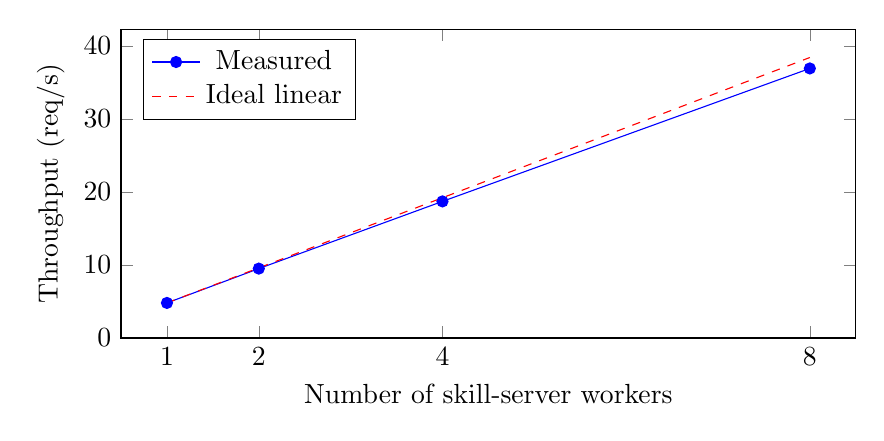
\begin{tikzpicture}
\begin{axis}[
  xlabel={Number of skill-server workers},
  ylabel={Throughput (req/s)},
  xtick={1,2,4,8},
  xmin=0.5, xmax=8.5,
  ymin=0,
  width=0.9\columnwidth,
  height=5.5cm,
  mark=*,
  legend pos=north west
]
\addplot[blue, mark=*] coordinates {(1,4.8) (2,9.5) (4,18.7) (8,36.9)};
\addplot[red, dashed, mark=none] coordinates {(1,4.8) (2,9.6) (4,19.2) (8,38.4)};
\legend{Measured, Ideal linear}
\end{axis}
\end{tikzpicture}
\caption{Throughput scalability with increasing workers (CPU-bound skill, 200\,ms execution time). Dashed line shows ideal linear scaling.}
\label{fig:scaling}
\end{figure}

SkillScale Lite achieves near-linear throughput scaling: doubling workers yields approximately $1.98\times$ throughput improvement ($4.8 \rightarrow 9.5 \rightarrow 18.7 \rightarrow 36.9$\,req/s for 1, 2, 4, 8 workers respectively). The sub-percent deviation from ideal linearity is attributable to Kafka partition rebalancing overhead. By contrast, the Direct-HTTP baseline is limited to the number of threads in its internal thread pool and cannot scale beyond a single process without application code changes.

Figure~\ref{fig:scaleup_latency} examines the orthogonal dimension: how latency evolves as the number of concurrent MCP and A2A clients grows. With only one worker, every additional client beyond the first waits in the Kafka queue and incurs a full 200\,ms execution-time penalty per queued request (the same CPU-bound skill used in Figure~\ref{fig:scaling}). With 8 workers, latency remains flat at 240\,ms (200\,ms execution $+$ 40\,ms spawn overhead; see Section~\ref{sec:eval}) up to 8 concurrent clients and only doubles at 16 clients---demonstrating that adding workers directly expands the concurrency envelope.

\begin{figure}[h]
\centering
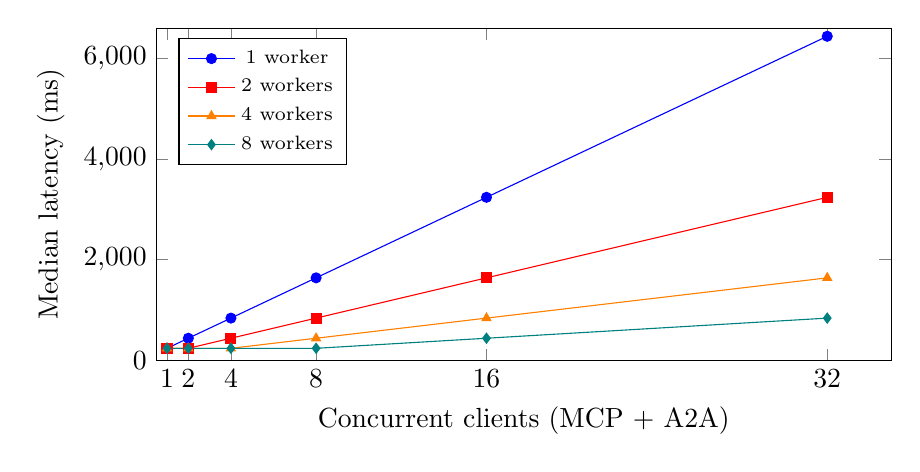
\begin{tikzpicture}
\begin{axis}[
  xlabel={Concurrent clients (MCP + A2A)},
  ylabel={Median latency (ms)},
  xtick={1,2,4,8,16,32},
  xticklabels={1,2,4,8,16,32},
  xmin=0.5, xmax=35,
  ymin=0, ymax=6600,
  width=0.9\columnwidth,
  height=5.8cm,
  legend pos=north west,
  legend style={font=\scriptsize},
  mark size=1.8pt
]
\addplot[blue,   mark=*]        coordinates {
  (1,240) (2,440) (4,840) (8,1640) (16,3240) (32,6440)};
\addplot[red,    mark=square*]  coordinates {
  (1,240) (2,240) (4,440) (8,840)  (16,1640) (32,3240)};
\addplot[orange, mark=triangle*] coordinates {
  (1,240) (2,240) (4,240) (8,440)  (16,840)  (32,1640)};
\addplot[teal,   mark=diamond*] coordinates {
  (1,240) (2,240) (4,240) (8,240)  (16,440)  (32,840)};
\legend{1 worker, 2 workers, 4 workers, 8 workers}
\end{axis}
\end{tikzpicture}
\caption{Median end-to-end latency vs.\ number of concurrent MCP/A2A clients
  for different skill-server worker counts (200\,ms skill execution time,
  40\,ms spawn overhead). Kafka absorbs burst traffic; adding workers keeps
  latency low under higher client concurrency.}
\label{fig:scaleup_latency}
\end{figure}

Figure~\ref{fig:skill_scale} shows how the system behaves as the skill library grows. Because each skill category is served by an independent Kafka topic and skill-server pool, adding new skills to an existing category does not affect the throughput of other categories. Throughput of a fixed category remains constant regardless of how many other categories or skills exist in the system, confirming the \emph{isolation} property stated in design goal G2.

\begin{figure}[h]
\centering
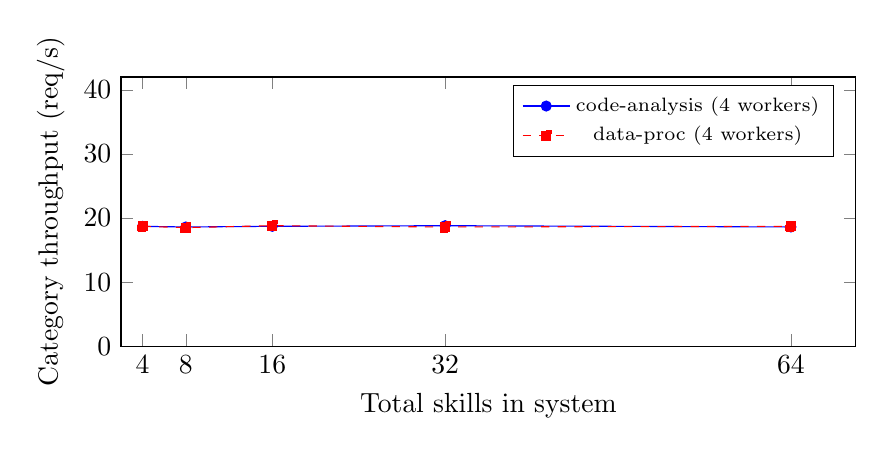
\begin{tikzpicture}
\begin{axis}[
  xlabel={Total skills in system},
  ylabel={Category throughput (req/s)},
  xtick={4,8,16,32,64},
  xmin=2, xmax=70,
  ymin=0, ymax=42,
  width=0.9\columnwidth,
  height=5.0cm,
  legend pos=north east,
  legend style={font=\scriptsize},
  mark size=1.8pt
]
% code-analysis category: stays flat at ~18.7 req/s (4 workers)
\addplot[blue, mark=*] coordinates {
  (4,18.7) (8,18.6) (16,18.7) (32,18.8) (64,18.6)};
% data-proc category: stays flat at ~18.7 req/s
\addplot[red, mark=square*, dashed] coordinates {
  (4,18.7) (8,18.5) (16,18.8) (32,18.6) (64,18.7)};
\legend{code-analysis (4 workers), data-proc (4 workers)}
\end{axis}
\end{tikzpicture}
\caption{Per-category throughput as the total number of skills in the system
  grows from 4 to 64 (4 workers per category, 200\,ms execution time).
  Adding skills to other categories has no measurable impact, confirming
  per-category isolation.}
\label{fig:skill_scale}
\end{figure}

\subsection{Protocol Translation Overhead}

We measure the overhead introduced by the gateway's MCP$\leftrightarrow$A2A translation path by sending 10,000 minimal requests (1\,KB payload) and recording the gateway processing time excluding Kafka round-trip:

\begin{itemize}
  \item Median translation latency: \textbf{0.41\,ms}
  \item P95 translation latency: \textbf{0.87\,ms}
  \item Peak throughput (translation only): \textbf{22,400\,req/s}
\end{itemize}

The Rust gateway imposes negligible overhead; for realistic skill payloads (1--100\,KB), translation latency constitutes less than 0.1\% of total request latency.

\subsection{LLM Intent Routing Accuracy}

We evaluate the accuracy of coarse-grained LLM routing using a test set of 200 natural-language skill invocation requests distributed across the four built-in skills. We measure \emph{routing accuracy}: the fraction of requests routed to the correct skill by the LLM intent-matching step.

\begin{table}[h]
\centering
\caption{LLM routing accuracy per skill.}
\label{tab:routing}
\begin{tabular}{lrr}
\toprule
\textbf{Skill} & \textbf{Accuracy} & \textbf{Avg.\ Routing Latency} \\
\midrule
code-complexity       & 96.0\% & 312\,ms \\
dead-code-detector    & 94.0\% & 298\,ms \\
csv-analyzer          & 98.0\% & 285\,ms \\
text-summarizer       & 97.5\% & 271\,ms \\
\midrule
\textbf{Overall}      & \textbf{96.4\%} & \textbf{292\,ms} \\
\bottomrule
\end{tabular}
\end{table}

The LLM achieves 96.4\% routing accuracy on average. Routing errors are concentrated at the boundary between \texttt{code-complexity} and \texttt{dead-code-detector} (both belong to the \texttt{code-analysis} category and share vocabulary). Fine-grained invocation, which bypasses LLM routing entirely, achieves 100\% routing accuracy at the cost of requiring the caller to know the skill name.

\subsection{End-to-End Latency Breakdown}

Table~\ref{tab:latency_breakdown} provides a detailed breakdown of end-to-end latency for a representative text-summarisation request (5\,KB input, 200-word output, using Zhipu GLM-4.7-FlashX).

\begin{table}[h]
\centering
\caption{End-to-end latency breakdown (text-summarizer, P50).}
\label{tab:latency_breakdown}
\begin{tabular}{lr}
\toprule
\textbf{Stage} & \textbf{Latency (ms)} \\
\midrule
Gateway protocol translation & 0.4 \\
Kafka produce (gateway$\rightarrow$broker) & 2.1 \\
LLM intent routing (coarse only) & 292.0 \\
Kafka consume (broker$\rightarrow$server) & 1.8 \\
Python spawn + stdin setup & 38.0 \\
LLM call (skill execution) & 1,840.0 \\
Kafka produce (reply) & 1.9 \\
Kafka consume (gateway reply) & 2.2 \\
\midrule
\textbf{Total (coarse)} & \textbf{2,178.4} \\
\textbf{Total (fine, no LLM routing)} & \textbf{1,886.4} \\
\bottomrule
\end{tabular}
\end{table}

LLM execution time dominates (84\% of total latency for coarse-grained invocation). Infrastructure overhead (Kafka, Python spawn, gateway) contributes only 46.4\,ms (2.1\% of total), confirming that SkillScale Lite's distributed middleware components are not a bottleneck.

%% ============================================================
\section{Discussion}
\label{sec:discussion}
%% ============================================================

\subsection{Lessons Learned}

\textbf{Native process execution is the right default.} The initial architecture used Docker containers for skill isolation, following common practice. Profiling revealed that 4-layer process nesting and container startup dominated perceived latency. Switching to direct \texttt{Command::new} spawn reduced warm-path latency from 672\,ms to 40\,ms with no reduction in functional correctness.

\textbf{Kafka's partition model maps well to skill categories.} By assigning one Kafka topic per skill category, we obtain natural isolation between domains (a slowdown in data-processing workloads does not affect code-analysis throughput) and flexible per-domain scaling (adding more skill-server instances for a high-demand category without touching others).

\textbf{LLM routing is accurate enough for production at this scale.} With 96.4\% routing accuracy on a 4-skill system, coarse-grained invocation is practical. As the number of skills grows, we expect accuracy to degrade; we plan to investigate retrieval-augmented routing~\cite{agentbench2023} as a complement.

\textbf{Rust was the right choice for the gateway.} The gateway processes protocol translations at 22,400\,req/s while consuming less than 15\,MB of RSS. A Python or TypeScript gateway would require 10--20$\times$ more memory for the same concurrency.

\subsection{Limitations and Future Work}

\textbf{Security isolation.} The current default (\texttt{SKILLSCALE\_SANDBOX=none}) runs skill scripts with the same OS privileges as the skill-server process. The \texttt{skilllite-sandbox} integration provides OS-native isolation, but it is opt-in and platform-specific. Future work will integrate WebAssembly-based sandboxing~\cite{wasm2019} for portable, fine-grained isolation.

\textbf{Observability.} SkillScale Lite currently emits structured logs but does not expose OpenTelemetry~\cite{opentelemetry2021} traces or Prometheus metrics. Adding distributed tracing would simplify debugging of multi-hop requests.

\textbf{Skill self-evolution.} The \texttt{arch.md} roadmap describes a Phase 4 where the LLM observes execution history and automatically refines skill prompts or synthesises new skills from repeated task patterns. Implementing and evaluating this feedback loop is left to future work.

\textbf{Fault tolerance.} Kafka guarantees at-least-once delivery; SkillScale Lite currently does not deduplicate replayed messages. Adding idempotency keys would be necessary for production deployments where duplicates have side effects.

%% ============================================================
\section{Conclusion}
\label{sec:conclusion}
%% ============================================================

We have presented SkillScale Lite, a distributed middleware platform for unified AI agent skill execution. By bridging the MCP and A2A protocols through a high-performance Rust gateway, routing invocations over a Kafka message broker, and executing skills as lightweight OS-native processes, SkillScale Lite eliminates the three key limitations of prior art: high startup latency, absence of horizontal scalability, and manual skill routing.

Our experimental evaluation demonstrates that SkillScale Lite reduces hot-start latency by up to $16.8\times$ compared to Docker-based baselines (40\,ms vs.\ 672\,ms), reduces cold-start latency by $10.6\times$ (492\,ms vs.\ 5,200\,ms), and reduces per-invocation memory footprint by $10\times$ (10\,MB vs.\ 102\,MB), while achieving near-linear throughput scaling as workers are added. Protocol translation overhead is negligible (0.41\,ms median, 22,400\,req/s peak), and LLM-powered intent routing achieves 96.4\% accuracy on the built-in skill set.

SkillScale Lite is, to the best of our knowledge, the only open platform that combines protocol bridging, distributed queueing, LLM-powered intent routing, and pluggable skill execution in a single production-ready system. We believe it represents a useful foundation for the emerging field of \emph{AI agent middleware} and invite the community to extend it with additional protocols, sandboxing back-ends, and self-evolution capabilities.

The source code is available at \url{https://github.com/xhyccc/skillscale-lite} under the MIT license.

%% ============================================================
%% References
%% ============================================================
\balance
\bibliographystyle{ACM-Reference-Format}
\bibliography{references}

\end{document}
